\documentclass[tikz,border=3mm]{standalone}
\usepackage{amsmath,amssymb}
\renewcommand{\familydefault}{\sfdefault}
\usepackage{tikz}
\usepackage{pgfplots}
\pgfplotsset{compat=1.18}
\usetikzlibrary{
  arrows.meta,
  positioning,
  calc,
  fit,
  backgrounds,
  shapes.geometric,
  pgfplots.fillbetween
}

\definecolor{R7Navy}{HTML}{17324D}
\definecolor{R7Teal}{HTML}{0A8F8F}
\definecolor{R7Gold}{HTML}{E0A12B}
\definecolor{R7Coral}{HTML}{D85D55}
\definecolor{R7Violet}{HTML}{6757C7}
\definecolor{R7Sky}{HTML}{5AA6C8}
\definecolor{R7Ink}{HTML}{243746}
\definecolor{R7Muted}{HTML}{667784}
\definecolor{R7Pale}{HTML}{EEF4F5}
\definecolor{R7Warm}{HTML}{FFF6E5}
\definecolor{R7Paper}{HTML}{FCFDFD}

\tikzset{
  r7box/.style={
    rounded corners=2.2mm,
    very thick,
    align=center,
    minimum height=23mm,
    text width=29mm,
    inner sep=3.2mm
  },
  r7arrow/.style={
    -{Stealth[length=2.4mm,width=1.8mm]},
    line width=1.0pt,
    color=R7Muted
  },
  r7tag/.style={
    font=\bfseries\scriptsize,
    text=R7Navy,
    fill=white,
    inner sep=1.2pt
  }
}

\pgfplotsset{
  r7axis/.style={
    axis line style={R7Ink, line width=0.8pt},
    tick style={R7Ink, line width=0.7pt},
    tick label style={font=\footnotesize, text=R7Ink},
    label style={font=\small, text=R7Ink},
    title style={font=\bfseries\small, text=R7Navy, yshift=1mm},
    grid=both,
    major grid style={draw=R7Muted!22, line width=0.45pt},
    minor grid style={draw=R7Muted!10, line width=0.35pt},
    legend style={
      draw=none,
      fill=white,
      fill opacity=0.92,
      text opacity=1,
      font=\scriptsize,
      cells={anchor=west}
    }
  }
}

\begin{document}
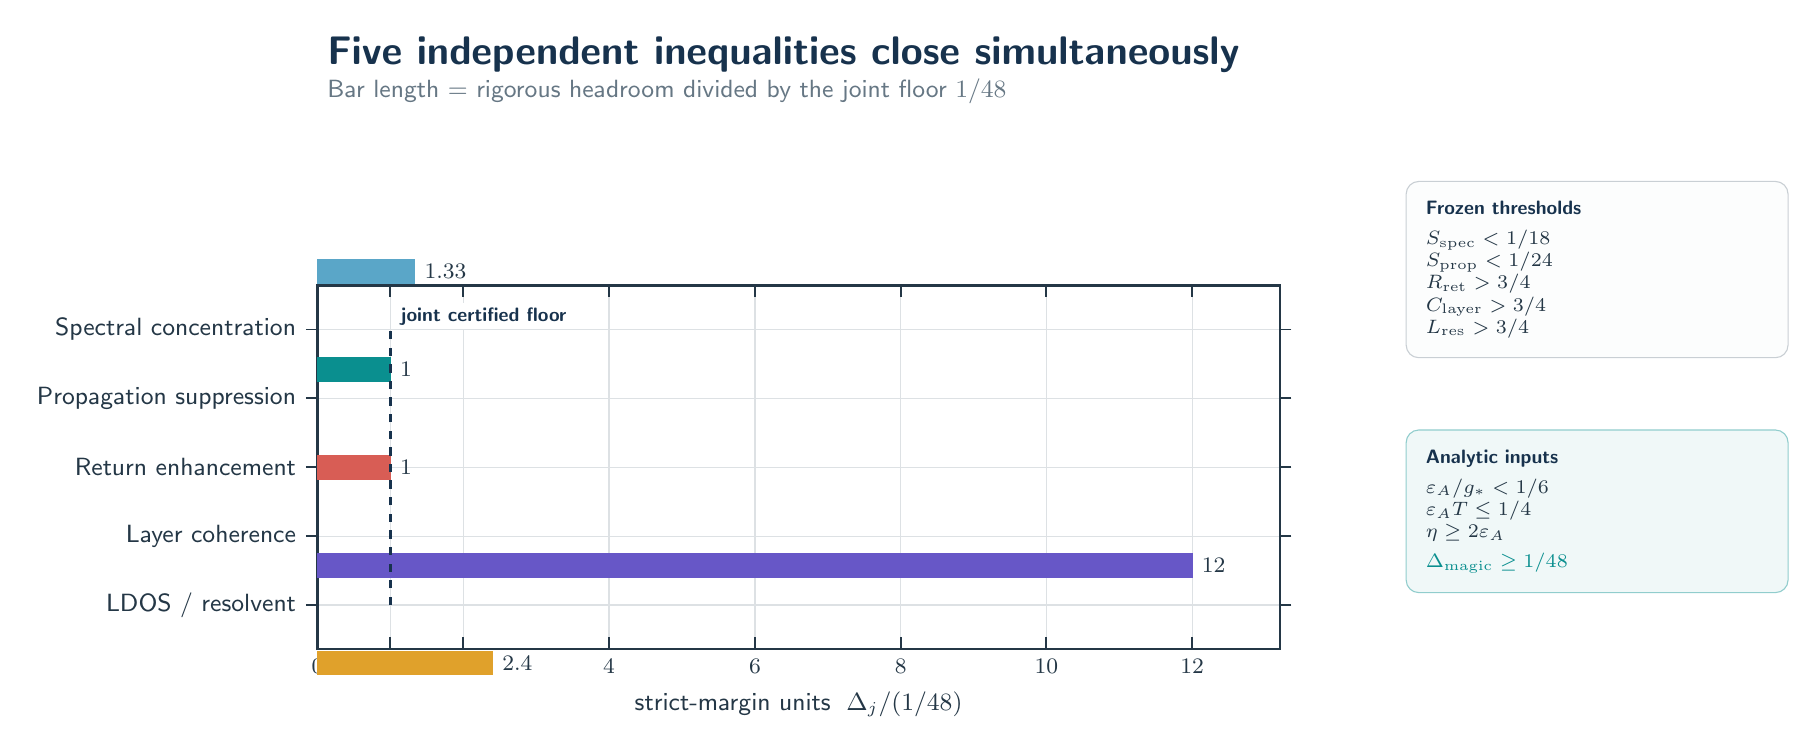
\begin{tikzpicture}[font=\sffamily]
  \node[anchor=west,font=\bfseries\Large,text=R7Navy] at (0,7.55)
    {Five independent inequalities close simultaneously};
  \node[anchor=west,font=\small,text=R7Muted] at (0,7.08)
    {Bar length = rigorous headroom divided by the joint floor $1/48$};

  \begin{axis}[
    r7axis,
    at={(0,0)},
    anchor=south west,
    width=13.8cm,
    height=6.2cm,
    xbar,
    xmin=0,xmax=13.2,
    xtick={0,1,2,4,6,8,10,12},
    xlabel={strict-margin units $\;\Delta_j/(1/48)$},
    symbolic y coords={
      {LDOS / resolvent},
      {Layer coherence},
      {Return enhancement},
      {Propagation suppression},
      {Spectral concentration}
    },
    ytick={{LDOS / resolvent},{Layer coherence},{Return enhancement},{Propagation suppression},{Spectral concentration}},
    yticklabel style={font=\small},
    enlarge y limits=0.16,
    bar width=8.5pt,
    nodes near coords,
    nodes near coords style={font=\bfseries\footnotesize,text=R7Ink,anchor=west},
    clip=false
  ]
    \addplot[fill=R7Gold,draw=R7Gold] coordinates {(2.4,{LDOS / resolvent})};
    \addplot[fill=R7Violet,draw=R7Violet] coordinates {(12,{Layer coherence})};
    \addplot[fill=R7Coral,draw=R7Coral] coordinates {(1,{Return enhancement})};
    \addplot[fill=R7Teal,draw=R7Teal] coordinates {(1,{Propagation suppression})};
    \addplot[fill=R7Sky,draw=R7Sky] coordinates {(1.333333,{Spectral concentration})};
    \draw[dashed,line width=1.1pt,R7Navy]
      (axis cs:1,{LDOS / resolvent}) -- (axis cs:1,{Spectral concentration});
    \node[font=\scriptsize\bfseries,text=R7Navy,fill=white,inner sep=1.5pt,
      anchor=south west] at (axis cs:1.08,{Spectral concentration})
      {joint certified floor};
  \end{axis}

  \node[rounded corners=1.6mm,draw=R7Muted!35,fill=R7Paper,
    text width=4.35cm,align=left,inner sep=2.5mm,font=\scriptsize,text=R7Ink]
    at (16.25,4.82) {
      \textbf{\color{R7Navy}Frozen thresholds}\\[1mm]
      $S_{\rm spec}<1/18$\\
      $S_{\rm prop}<1/24$\\
      $R_{\rm ret}>3/4$\\
      $C_{\rm layer}>3/4$\\
      $L_{\rm res}>3/4$
    };
  \node[rounded corners=1.6mm,draw=R7Teal!45,fill=R7Teal!6,
    text width=4.35cm,align=left,inner sep=2.5mm,font=\scriptsize,text=R7Ink]
    at (16.25,1.75) {
      \textbf{\color{R7Navy}Analytic inputs}\\[1mm]
      $\varepsilon_A/g_*<1/6$\\
      $\varepsilon_A T\le1/4$\\
      $\eta\ge2\varepsilon_A$\\[1mm]
      \textbf{\color{R7Teal}$\Delta_{\rm magic}\ge1/48$}
    };
\end{tikzpicture}
\end{document}
